\subsection{Cache Organization}
\label{sec:cache_org}

In the Intel architecture, caches are completely implemented in hardware,
meaning that the software stack has no control over the eviction process.
However, software can gain some control over which data gets evicted by
understanding how the caches are organized, and by cleverly placing its data in
memory. This knowledge can be used to mount a cache timing attack, and it can
also be used by system software to protect the software it manages from cache
timing attacks.

The \textit{cache line} is the atomic unit of cache organization. A cache line
has \textit{data}, a copy of a continuous range of DRAM, and a \textit{tag},
identifying the memory address that the data comes from. Fills and evictions
are performed on entire lines.

The cache line size is the size of the data, and is always a power of two.
Assuming $n$-bit memory addresses and a cache line size of $2^{l}$ bytes, the
lowest $l$ bits of a memory address are an offset into a cache line, and the
highest $n - l$ bits determine the cache line that is used to store the data at
the memory location. All recent processors have 64-byte cache lines.

The L1 and L2 caches in recent processors are multi-way set-associative with
direct set indexing, as shown in Figure~\ref{fig:cpu_cache}. A $W$-way
set-associative cache has its memory divided into \textit{sets}, where each set
has $W$ lines. A memory location can be cached in any of the $w$ lines in a
specific set that is determined by the highest $n - l$ bits of the location's
memory address. Direct set indexing means that the $S$ sets in a cache are
numbered from $0$ to $S - 1$, and the memory location at address $A$ is cached
in the set numbered $A_{n - 1 \ldots n - l} \bmod S$.

In the common case where the number of sets in a cache is a power of two, so $S
= 2^{s}$, the lowest $l$ bits in an address make up the cache line offset, the
next $s$ bits are the set index. The highest $n - s - l$ bits in an address are
not used when selecting where a memory location will be cached.
Figure~\ref{fig:cpu_cache} shows the cache structure and lookup process.

\begin{figure}[hbt]
  \centering
  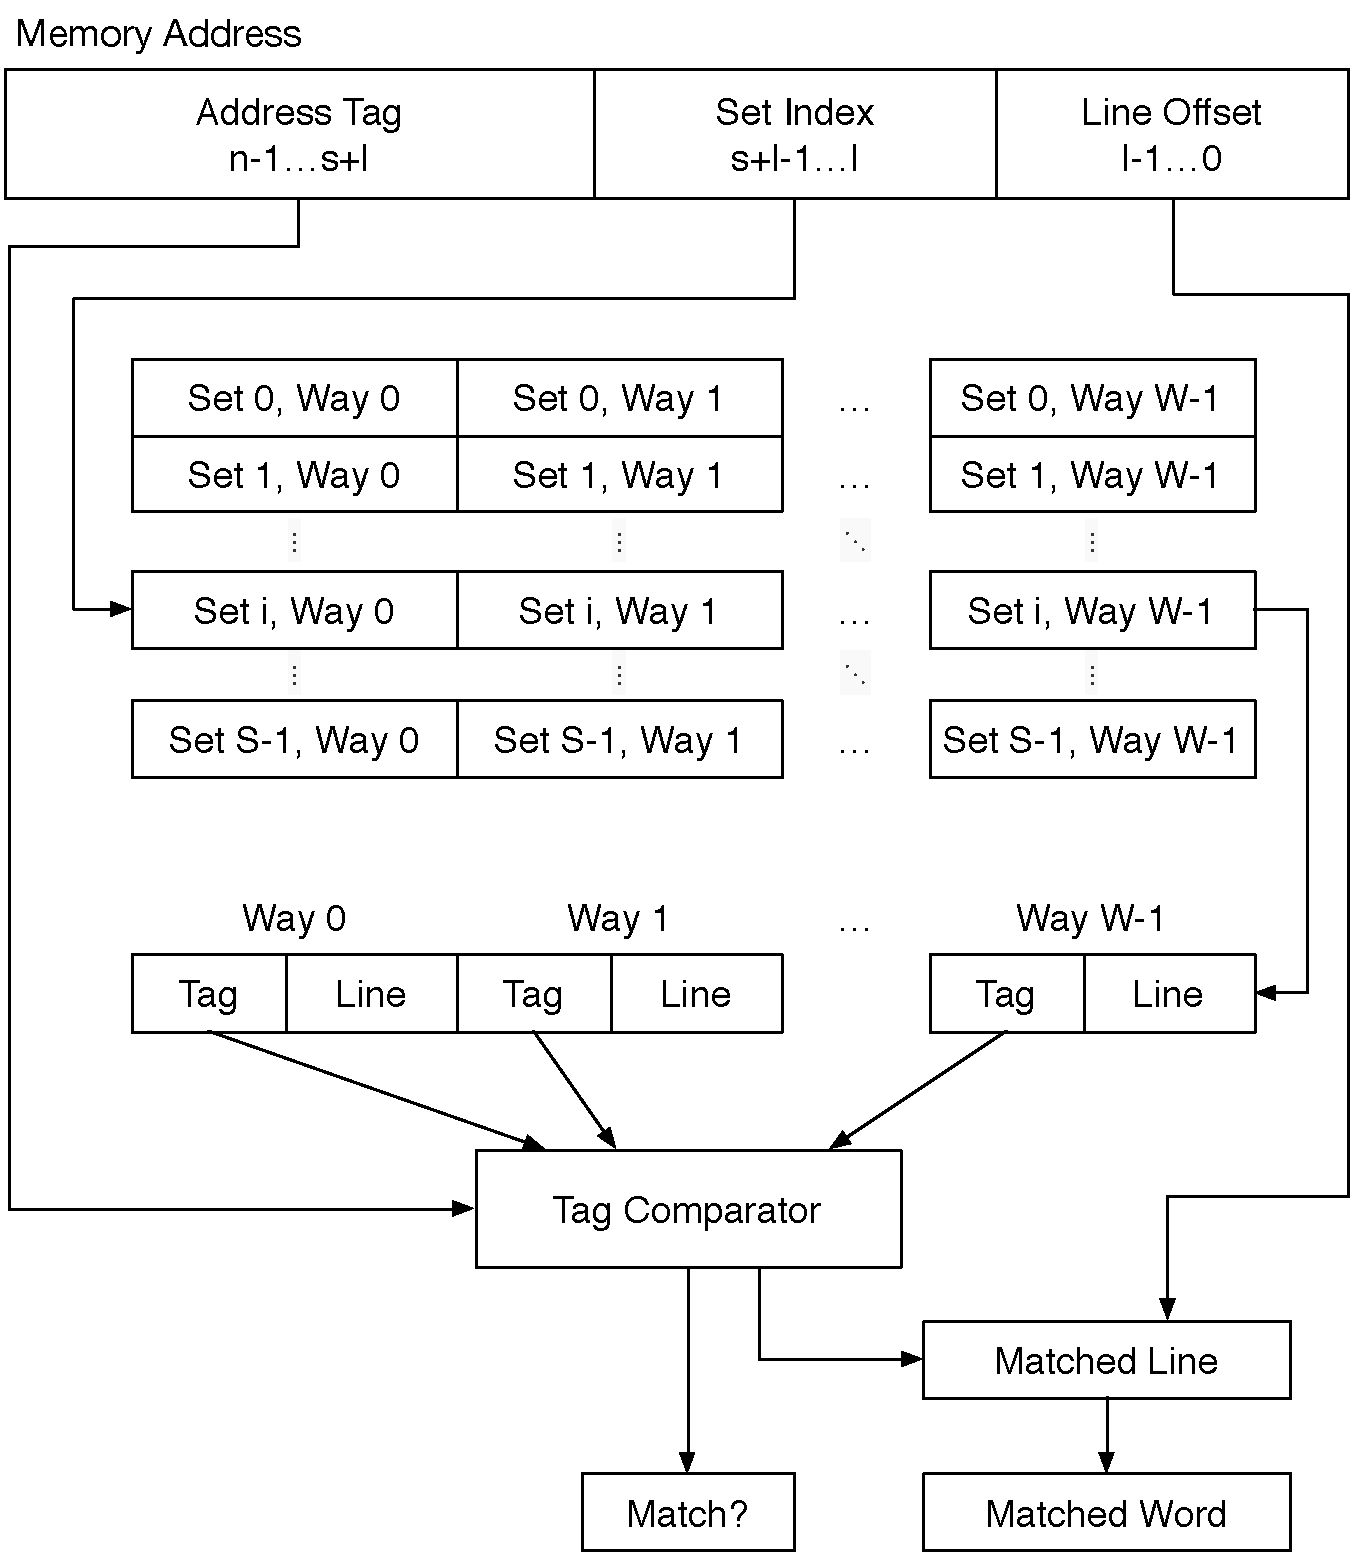
\includegraphics[width=85mm]{figures/cpu_cache.pdf}
  \caption{
    Cache organization and lookup, for a $W$-way set-associative cache with
    $2^{l}$-byte lines and $S = 2^{s}$ sets. The cache works with $n$-bit
    memory addresses. The lowest $l$ address bits point to a specific byte in a
    cache line, the next $s$ bytes index the set, and the highest $n - s - l$
    bits are used to decide if the desired address is in one of the $W$ lines
    in the indexed set.
  }
  \label{fig:cpu_cache}
\end{figure}
